%%%%%%%%%%%%%%%%%%%%%%%%%%%%%%%%%%%%%%%%%%%%%%%%%%%%%%%%
%%%%%%%%%%%%%%%%%%%%%%%%%%%%%%%%%%%%%%%%%%%%%%%%%%%%%%%%
%%%%%%%%%%%%%%%%%%%%%%%%%%%%%%%%%%%%%%%%%%%%%%%%%%%%%%%%
\chapter{Hypothesis Testing}
\label{chap:hypo}

%%%%%%%%%%%%%%%%%%%%%%%%%%%%%%%%%%%%%%%%%%%%%%%%%%%%%%%%
%%%%%%%%%%%%%%%%%%%%%%%%%%%%%%%%%%%%%%%%%%%%%%%%%%%%%%%%
\section{Hypothesis Test Selection}
\label{hypo:test_selection}
% TODO

%%%%%%%%%%%%%%%%%%%%%%%%%%%%%%%%%%%%%%%%%%%%%%%%%%%%%%%%
%%%%%%%%%%%%%%%%%%%%%%%%%%%%%%%%%%%%%%%%%%%%%%%%%%%%%%%%
\section{\texorpdfstring{$Z$}{Z}-Test}
\label{hypo:Z_test}

When we sample from a distribution known to be Gaussian,
or can assume the sample means are approximately normally distributed via the central limit theorem (CLT) of \cref{stats:CLT},
and know the population standard deviation $\sigma$,
we can perform hypothesis testing on the sample mean with a \Ztest.
For a sample of size $n$ with sample mean $\expval{x}$ and population standard deviation $\sigma$
we compute the \Zscore,

\begin{equation}\label{eq:hypo:Z}
Z = \frac{\expval{x} - \mu_{0}}{\sigma_{\expval{x}}} = \frac{\expval{x} - \mu_{0}}{\sigma/\sqrt{n}},
\end{equation}

\noindent and test the null hypothesis, $H_{0}$, that the mean is $\mu_{0}$
by comparing $Z$ to the standard normal distribution.
Depending on if we wish to perform a one-sided or two-sided
test\footnote{Note we can also perform two-sample and paired {\Ztest}s, see the analogous \ttest sections with $\sigma$ replacing $s$.} we
find the probability of observing $P\left(x < Z\right)$, $P\left(Z < x\right)$, or $P\left(Z < \abs{x}\right)$
from the cumulative distribution function (CDF).
This \pvalue then determines if we accept, $\pvalue < \alpha$, or reject, $\alpha \leq \pvalue$,
$H_{0}$ at a given significance level $\alpha$, typically \num{0.05} or lower.
We can
\href{https://docs.scipy.org/doc/scipy/reference/generated/scipy.stats.zscore.html}{compute $Z$} with
\texttt{scipy.stats.zscore},
and \href{https://docs.scipy.org/doc/scipy/reference/generated/scipy.stats.norm.html}{find the \pvalue} with
\texttt{scipy.stats.norm.cdf} or \texttt{scipy.stats.norm.sf},
being careful to include the correct side(s).
For an illustration see \cref{fig:two_sided_t_test}, with \Zscore replacing the \tstat.

If we do not know the population standard deviation $\sigma$, as is often the case,
or if $n \lesssim 30$, we should use a \ttest instead.
However, if $50 \lesssim n$ we may be able to approximate $\sigma \approx s$
and use a \Ztest anyway.

%%%%%%%%%%%%%%%%%%%%%%%%%%%%%%%%%%%%%%%%%%%%%%%%%%%%%%%%
%%%%%%%%%%%%%%%%%%%%%%%%%%%%%%%%%%%%%%%%%%%%%%%%%%%%%%%%
\section{Student's \texorpdfstring{$t$}{t}-Test}
\label{hypo:t_test}

Student's \ttest can be used to
statistically compare the means of two samples via the \tdist
given a \tstat and degrees of freedom $\nu$.
The \ttest is appropriate when each sample is small\footnote{For
larger sample sizes the \tdist approaches the normal distribution which should be used instead.}, $n \lesssim 30$,
and drawn from a larger normally distributed population with an unknown standard deviation.
The \pvalue returned by the test estimates the probability of obtaining the sample means
assuming $H_{0}$, typically that the samples share the same mean, is true.
We can compute two-sided, \ie the means are not equal, or one-sided, \ie mean 1 is $>$ or $<$ mean 2,
forms of the \ttest in three basic variations.
See \cref{fig:two_sided_t_test} for an illustration of a two-sided test's $H_{0}$ rejection regions.
The \texttt{scipy.stats.ttest\_*}
\href{https://docs.scipy.org/doc/scipy/reference/stats.html#statistical-tests}{family of functions}
make it easily to compute {\tstat}s and {\pvalue}s in practice.

\begin{figure}
\centering
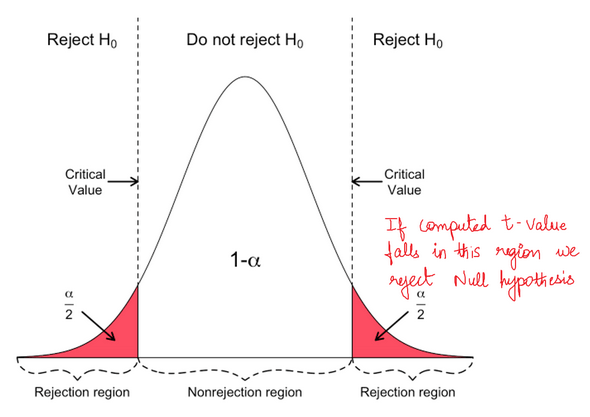
\includegraphics[width=0.7\textwidth]{figures/stats/one_side_t_test_rejection_regions.png}
\caption{
Illustration of a two-sided {\ttest}'s null hypothesis, $H_{0}$, rejection regions,
by \href{https://www.machinelearningplus.com/statistics/t-test-students-understanding-the-math-and-how-it-works/}{Selva Prabhakaran}.
In a one-sided \ttest we would only consider the side on a single side.
$\alpha$ is the significance level, typically \num{0.05} or lower.
}
\label{fig:two_sided_t_test}
\end{figure}

%%%%%%%%%%%%%%%%%%%%%%%%%%%%%%%%%%%%%%%%%%%%%%%%%%%%%%%%
\subsection{One-Sample}
\label{hypo:t_test:one}

In a one-sample \ttest we have one sample of size $n$ with mean $\expval{x}$ and standard deviation $s$,
and test $H_{0}$ that it belongs to a parent population with mean $\mu_{0}$.
In this case the parent population does not need to be normally distributed, but the distribution of possible $\expval{x}$ is assumed to be normal.

The \tstat \cref{eq:hypo:t:one} can be used with $\nu = n-1$ to find a \pvalue.

\begin{equation}\label{eq:hypo:t:one}
t = \frac{\expval{x} - \mu_{0}}{s / \sqrt{n}}
\end{equation}

%%%%%%%%%%%%%%%%%%%%%%%%%%%%%%%%%%%%%%%%%%%%%%%%%%%%%%%%
\subsection{Two-Sample: Unpaired}
\label{hypo:t_test:two:unpaired}

In a two-sample unpaired \ttest we have two independent samples, each of size $n$,
but with their own sample means $\expval{x_{i}}$ and standard deviations $s_{i}$.
Provided that we can assume that the two parent distributions of $x_{1}$ and $x_{2}$ have the same variance,
we can test $H_{0}$ that the two parent distribution means are equal.

The \tstat \cref{eq:hypo:t:two:unpaired} can be used with $\nu = 2n-2$ to find a \pvalue.

\begin{subequations}\label{eq:hypo:t:two:unpaired}
\begin{align}
t &= \frac{\expval{x_{1}} - \expval{x_{2}}}{s_{p} \sqrt{2/n}} \label{eq:hypo:t:two:unpaired:t} \\
s_{p} &= \sqrt{\left(s^{2}_{x_{1}} + s^{2}_{x_{2}}\right)/2} \label{eq:hypo:t:two:unpaired:s_p}
\end{align}
\end{subequations}

\subsubsection{Different Sample Sizes}
\label{hypo:t_test:two:unpaired:diff_n}

If we relax the sample size condition and let $n_{1} \neq n_{2}$
we can still compute a \tstat,
provided the parent distribution's variances are equal\footnote{A useful guideline is $1/2 < s_{x_{1}} / s_{x_{2}} < 2$.}.

The \tstat \cref{eq:hypo:t:two:unpaired:diff_n} can be used with $\nu = n_{1} + n_{2} - 2$ to find a \pvalue.

\begin{subequations}\label{eq:hypo:t:two:unpaired:diff_n}
\begin{align}
t &= \frac{\expval{x_{1}} - \expval{x_{2}}}{s_{p} \sqrt{\frac{1}{n_{1}} + \frac{1}{n_{2}}}} \label{eq:hypo:t:two:unpaired:diff_n:t} \\
s_{p} &= \sqrt{\left(\left(n_{1} - 1\right)s^{2}_{x_{1}} + \left(n_{2} - 1\right)s^{2}_{x_{2}}\right)/\left(n_{1} + n_{2} -2\right)} \label{eq:hypo:t:two:unpaired:diff_n:s_p}
\end{align}
\end{subequations}

\subsubsection{Different Sample Sizes and Variances (Welch's \texorpdfstring{$t$}{t}-Test)}
\label{hypo:t_test:two:unpaired:diff_n_diff_var}

If we further relax the assumptions and also let the population variances differ
we arrive at Welch's \ttest which approximates\footnote{The
true distribution of $t$ depends somewhat on the unknown population variances,
see the \href{https://en.wikipedia.org/wiki/Behrens\%E2\%80\%93Fisher_problem}{Behrens--Fisher problem}
for more.} the \tdist.

The \tstat \cref{eq:hypo:t:two:unpaired:diff_n_diff_var:t} can be used with $\nu$ \cref{eq:hypo:t:two:unpaired:diff_n_diff_var:dof} to find a \pvalue.

\begin{subequations}\label{eq:hypo:t:two:unpaired:diff_n_diff_var}
\begin{align}
t &= \frac{\expval{x_{1}} - \expval{x_{2}}}{\sqrt{\frac{s^{2}_{1}}{n_{1}} + \frac{s^{2}_{2}}{n_{2}}}} \label{eq:hypo:t:two:unpaired:diff_n_diff_var:t} \\
\nu &= \frac{\left(s^{2}_{1}/n_{1} + s^{2}_{2}/n_{2}\right)^{2}}{\frac{\left(s^{2}_{1}/n_{1}\right)^{2}}{n_{1}-1} + \frac{\left(s^{2}_{2}/n_{2}\right)^{2}}{n_{2}-1}} \label{eq:hypo:t:two:unpaired:diff_n_diff_var:dof}
\end{align}
\end{subequations}

%%%%%%%%%%%%%%%%%%%%%%%%%%%%%%%%%%%%%%%%%%%%%%%%%%%%%%%%
\subsection{Two-Sample: Paired}
\label{hypo:t_test:two:paired}

In a two-sample paired \ttest we have two dependent samples,
such as two sets of measurements from the same $n$ individuals taken at different times.
In this case, we are testing $H_{0}$ that the difference in means of the two dependent samples is $\mu_{0}$.
Note, we can set $\mu_{0} = 0$ if we simply want to test for a statistically significant difference, and not an \apriori degree of difference.
Defining the difference between paired observations as $x_{\Delta}$, we compute the mean difference $\expval{x_{\Delta}}$ and $s_{\Delta}$ standard deviation on the sample.

The \tstat \cref{eq:hypo:t:two:paired} can be used with $\nu = n-1$ to find a \pvalue.

\begin{equation}\label{eq:hypo:t:two:paired}
t = \frac{\expval{x_{\Delta}} - \mu_{0}}{s_{\Delta} / \sqrt{n}}
\end{equation}

%%%%%%%%%%%%%%%%%%%%%%%%%%%%%%%%%%%%%%%%%%%%%%%%%%%%%%%%
%%%%%%%%%%%%%%%%%%%%%%%%%%%%%%%%%%%%%%%%%%%%%%%%%%%%%%%%
\section{\texorpdfstring{$\chi^{2}$-Test}{Chi-Squared Test}}
\label{hypo:chi2_test}

Pearson's \chiSqtest can be used to
statistically compare a set of observations in
$n$ variables, $x_{i}$, to prior expectations via the \chiSqdist.
The \pvalue returned by the test estimates the probability of obtaining the observations
assuming $H_{0}$, \ie the expectations, is true.
The \chiSqstat, $X^{2}$, is created with the assumption that
the data are normally distributed and independent,
which often is the case due to the CLT.
It is constructed by squaring the difference\footnote{Yates's
correction for continuity $\left(x^{\text{obs}}_{j} - x^{\text{exp}}_{j}\right)^{2} \to \left(\abs{x^{\text{obs}}_{j} - x^{\text{exp}}_{j}}-0.5\right)^{2}$ may
also be applied in some low statistics cases.} between
an expected value, $x^{\text{exp}}_{i}$, and its corresponding observation, $x^{\text{obs}}_{i}$,
and dividing by the expectation:

\begin{equation}\label{eq:hypo:chi2_statistic}
X^{2} = \sum_{i=1}^{n} \frac{\left(x^{\text{obs}}_{i} - x^{\text{exp}}_{i}\right)^{2}}{x^{\text{exp}}_{i}}\,.
\end{equation}

In the limit that each $x^{\text{obs}}_{i}$ is normally distributed and $n$ is large, $X^{2} \to \chi^{2}$.
We can then use the \chiSqdist with $\nu = n-1$ degrees of freedom to find the \pvalue as the area to the right of $X^{2}$.
An easy way to compute $X^{2}$ and the \pvalue is to use the \texttt{scipy.stats.chisquare(f\_obs, f\_exp)}
\href{https://docs.scipy.org/doc/scipy/reference/generated/scipy.stats.chisquare.html}{function}.

The \chiSqtest can also be used to test of the data's independence, or homogeneity,
for $m$ samples of $n$ variables with $\nu = \left(n-1\right)\left(m-1\right)$ and\footnote{Note this is really the same as \cref{eq:hypo:chi2_statistic} if we reindex, just with a different $\nu$.}

\begin{equation}\label{eq:hypo:chi2_statistic_ind}
X^{2} = \sum_{i=1}^{n} \sum_{j=1}^{m} \frac{\left(x^{\text{obs}}_{i,j} - x^{\text{exp}}_{i,j}\right)^{2}}{x^{\text{exp}}_{i,j}}\,.
\end{equation}

%%%%%%%%%%%%%%%%%%%%%%%%%%%%%%%%%%%%%%%%%%%%%%%%%%%%%%%%
%%%%%%%%%%%%%%%%%%%%%%%%%%%%%%%%%%%%%%%%%%%%%%%%%%%%%%%%
\section{Analysis of Variance (ANOVA)}
\label{hypo:ANOVA}

When we are tasked with testing for differences between multiple groups
we should not use multiple pairwise tests, like two-sample unpaired {\ttest}s,
as the family-wise error rate \cref{eq:hypo:alpha_fw}
will compound and become unreasonable, see \cref{hypo:bonferroni_correction} for more.
Instead when dealing with three\footnote{When there are only two groups a one-factor ANOVA is equivalent to a two-sample unpaired \ttest with $F=t^{2}$.} or more groups
the appropriate Analysis of Variance (ANOVA) method should be used.
Like pairwise tests, there are multiple versions of ANOVA available for different situations, including
factorial ANOVA for multiple independent variables with interaction terms,
repeated measures ANOVA where the same subjects tested in different situations form the different groups,
Multivariate Analysis of Variance (MANOVA) for multiple dependent variables,
and further extensions such as Analysis of Covariance (ANCOVA) which incorporate correlations with additional covariate variables.
All share similar principles and assumptions,
but we will only focus on one-factor ANOVA here.

In general, ANOVA methods work by ``partitioning the sum of squares'',
\ie dividing the variance present in the data into
``explained variance'', \ie ``between-group variability'',
and
``unexplained variance'', \ie ``within-group variability'',
components.
The ratio of these components then form a \Fstat
which can be compared against the \Fdist
with the appropriate degrees of freedom to produce a \pvalue.
The null hypothesis $H_{0}$ is typically that all of the groups come from populations which share the same mean.
Increased between-group variability, or decreased within-group variability,
will increase the \Fstat and make rejecting $H_{0}$ more probable.
One downside to ANOVA testing is that if we reject $H_{0}$
we will not know which group(s) differ from the others.
In this case additional \posthoc analysis is required,
such as Bonferroni corrected {\ttest}s or Tukey's honest significance test.

%%%%%%%%%%%%%%%%%%%%%%%%%%%%%%%%%%%%%%%%%%%%%%%%%%%%%%%%
\subsection{Assumptions}
\label{hypo:ANOVA:assumptions}

Mathematically ANOVA is a special case of linear regression
and shares many of the same assumptions:

\begin{enumerate}[noitemsep]
  \item The variances of the different groups are equal (homoscedasticity).
  \item The observations $y_{ij}$ within group $i$ are independent and identically distributed (i.i.d.), normal random variables.
  \item The residuals are normally distributed (normality\footnote{The normality assumption can be bent without severe consequences, but as always review the literature for specifics first.}).
  \item The dependent variable is continuous.
\end{enumerate}

%%%%%%%%%%%%%%%%%%%%%%%%%%%%%%%%%%%%%%%%%%%%%%%%%%%%%%%%
\subsection{One-Factor}
\label{hypo:ANOVA:one}

A one-factor ANOVA should be used when comparing $K$ groups,
divided by a single independent variable $x$,
across a single dependent variable $y$.
We partition the sum of squares into
mean square $MS_{\text{between-group}}$ and $MS_{\text{within-group}}$
\cref{eq:hypo:ANOVA:one:MS_between,eq:hypo:ANOVA:one:MS_within}, where
$n_{i}$ represents the number of observations in the $i$th group,
$N = \sum_{i} n_{i}$ is the total number of observations,
$y_{ij}$ is the $j$th observation for group $i$,
$\expval{Y_{i}} = \sum_{j} y_{ij} / n_{i}$ is the mean for group $i$,
and $\expval{Y} = \sum_{i}\sum_{j} y_{ij} / N$ is the overall mean across all groups.

\begin{subequations}\label{eq:hypo:ANOVA:one}
\begin{align}
MS_{\text{between-group}} &= \frac{1}{K-1} \sum_{i=1}^{K} n_{i}\left(\expval{Y_{i}} - \expval{Y}\right)^{2}, \label{eq:hypo:ANOVA:one:MS_between} \\
MS_{\text{within-group}} &= \frac{1}{N-K} \sum_{i=1}^{K} \sum_{j=1}^{n_{i}} \left( y_{ij} - \expval{Y_{i}} \right)^{2}, \label{eq:hypo:ANOVA:one:MS_within} \\
F &= \frac{MS_{\text{between-group}}}{MS_{\text{within-group}}}, \label{eq:hypo:ANOVA:one:F} \\
d_{1} &= K-1,\quad d_{2} = N-K. \label{eq:hypo:ANOVA:one:dof}
\end{align}
\end{subequations}

Note that $MS_{\text{between-group}}$ is comparing the group means to the overall mean,
while $MS_{\text{within-group}}$ is comparing all of the data points to their respective group means.
The \Fstat is then the ratio of the mean squares \cref{eq:hypo:ANOVA:one:F},
which can be used with the appropriate degrees of freedom \cref{eq:hypo:ANOVA:one:dof}
and the \Fdist to produce a \pvalue.
Depending on the \pvalue and selected $\alpha$
we can accept or reject $H_{0}$,
\ie all of the groups share one mean.
The \texttt{scipy.stats.f\_oneway} \href{https://docs.scipy.org/doc/scipy/reference/generated/scipy.stats.f_oneway.html#scipy.stats.f_oneway}{function}
performs\footnote{See
\href{https://www.analyticsvidhya.com/blog/2020/06/introduction-anova-statistics-data-science-covid-python/}{here} and
\href{https://www.reneshbedre.com/blog/anova.html}{here}
for example implementations.} the one-factor ANOVA test.

%%%%%%%%%%%%%%%%%%%%%%%%%%%%%%%%%%%%%%%%%%%%%%%%%%%%%%%%
%%%%%%%%%%%%%%%%%%%%%%%%%%%%%%%%%%%%%%%%%%%%%%%%%%%%%%%%
\section{\texorpdfstring{$F$}{F}-Test of Equality of Variances}
\label{hypo:F_test_var}

We can test $H_{0}$ that the variances of two normally distributed samples are equal with a \Ftest.
Given two samples of sizes $n_{1}$ and $n_{2}$ with sample variances $s_{2}^{2} \leq s_{1}^{2}$
we construct the \Fstat as:

\begin{equation}\label{eq:hypo:F_test_var}
F = \frac{s_{1}^{2}}{s_{2}^{2}}\,.
\end{equation}

The \Fdist with degrees of freedom $d_{1} = n_{1}-1$ and $d_{2} = n_{2}-1$
then gives an appropriate \pvalue.
Note that this \Ftest is particularly sensitive to the assumption that
the underlying samples are truly normally distributed;
not only approximately normal via the CLT.

%%%%%%%%%%%%%%%%%%%%%%%%%%%%%%%%%%%%%%%%%%%%%%%%%%%%%%%%
%%%%%%%%%%%%%%%%%%%%%%%%%%%%%%%%%%%%%%%%%%%%%%%%%%%%%%%%
\section{Binomial Proportion Test}
\label{hypo:binomial_test}

When dealing with samples of $n$ binary events we can perform hypothesis testing
on the number of observed positive events $k$
using test statistics built on the binomial distribution.

%%%%%%%%%%%%%%%%%%%%%%%%%%%%%%%%%%%%%%%%%%%%%%%%%%%%%%%%
\subsection{Exact Binomial Test}
\label{hypo:binomial_test:exact}

For small $n$ it is possible to compute the \pvalue
explicitly from the binomial distribution \cref{eq:stats:binomial}.
We test $H_{0}$ that the probability of success is $\pi_{0}$
having actually observed $k$ successes, $k = n \pi$.

The \pvalue is then the sum

\begin{equation}\label{eq:hypo:binomial_test:exact}
\pvalue = \sum_{i \in \, \mathcal{I}} \binom{n}{i} \pi_{0}^{i} \left(1-\pi_{0}\right)^{n-i},
\end{equation}

\noindent where $\mathcal{I}$ depends on the type of test:

\begin{table}[H]
\centering
\begin{tabular}{l|l}
$\pi < \pi_{0}$ & $\mathcal{I} = \left\{0, 1, \ldots, k\right\}$, \\
$\pi > \pi_{0}$ & $\mathcal{I} = \left\{k, k+1, \ldots, n\right\}$, \\
$\pi \neq \pi_{0}$ & $\mathcal{I} = \left\{\forall \, i: P\left(x=i\right) \leq P\left(x = k\right)\right\}$, with binomial $P\left(x\right)$ \cref{eq:stats:binomial}.
\end{tabular}
\end{table}

%%%%%%%%%%%%%%%%%%%%%%%%%%%%%%%%%%%%%%%%%%%%%%%%%%%%%%%%
\subsection{One-Sample}
\label{hypo:binomial_test:one}

For large sample sizes the binomial distribution is approximated by the normal distribution
and we can use a form of the \Ztest to produce {\pvalue}s.
We require the observations to be independent,
\ie we may only sample $< \SI{10}{\percent}$ of the parent population,
the sampling distribution of $\pi$ to be approximately normal,
and that there are $\geq 10$ successes and $\geq 10$ failures,
$n \pi_{0} \geq 10$ and $n \left(1-\pi_{0}\right) \geq 10$, \ie the success-failure condition.

The \Zscore is then:

\begin{equation}\label{eq:hypo:binomial_test:one}
Z = \frac{\pi - \pi_{0}}{\sqrt{\pi_{0}\left(1-\pi_{0}\right)/n}} = \frac{k - n \pi_{0}}{\sqrt{n\pi_{0}\left(1-\pi_{0}\right)}}.
\end{equation}

Note that the one-sample test is provided by the
\texttt{scipy.stats.binomtest} \href{https://docs.scipy.org/doc/scipy/reference/generated/scipy.stats.binomtest.html}{function}.

%%%%%%%%%%%%%%%%%%%%%%%%%%%%%%%%%%%%%%%%%%%%%%%%%%%%%%%%
\subsection{Two-Sample}
\label{hypo:binomial_test:two}

In the case of two samples, we can test $H_{0}$
that the difference\footnote{Again, we set $\pi_{\Delta} = 0$ if we want to test for any difference.} in the sample's probabilities is $\pi_{\Delta}$.
We require that the $\pi$ from the two samples are uncorrelated,
have approximately normal sampling distributions,
and that their difference $\pi_{1} - \pi_{2}$ is an unbiased estimator.

The \Zscore is then:

\begin{subequations}\label{eq:hypo:binomial_test:two}
\begin{align}
Z &= \frac{\pi_{1} - \pi_{2} - \pi_{\Delta}}{\pi_{p} \left(1-\pi_{p}\right)\left(1/n_{1} + 1/n_{2}\right)} \label{eq:hypo:binomial_test:two:Z} \\
\pi_{p} &= \frac{k_{1} + k_{2}}{n_{1} + n_{2}} \label{eq:hypo:binomial_test:two:pi_p}
\end{align}
\end{subequations}

%%%%%%%%%%%%%%%%%%%%%%%%%%%%%%%%%%%%%%%%%%%%%%%%%%%%%%%%
%%%%%%%%%%%%%%%%%%%%%%%%%%%%%%%%%%%%%%%%%%%%%%%%%%%%%%%%
\section{Mann-Whitney \texorpdfstring{$U$}{U} Test}
\label{hypo:mann_whitney_U_test}
% TODO

%%%%%%%%%%%%%%%%%%%%%%%%%%%%%%%%%%%%%%%%%%%%%%%%%%%%%%%%
%%%%%%%%%%%%%%%%%%%%%%%%%%%%%%%%%%%%%%%%%%%%%%%%%%%%%%%%
\section{Kruskal-Wallis \texorpdfstring{$H$}{H} Test}
\label{hypo:kruskal_wallis_H_test}
% TODO

%%%%%%%%%%%%%%%%%%%%%%%%%%%%%%%%%%%%%%%%%%%%%%%%%%%%%%%%
%%%%%%%%%%%%%%%%%%%%%%%%%%%%%%%%%%%%%%%%%%%%%%%%%%%%%%%%
\section{Kolmogorov-Smirnov Test}
\label{hypo:KS_test}
% TODO

%%%%%%%%%%%%%%%%%%%%%%%%%%%%%%%%%%%%%%%%%%%%%%%%%%%%%%%%
%%%%%%%%%%%%%%%%%%%%%%%%%%%%%%%%%%%%%%%%%%%%%%%%%%%%%%%%
\section{Hypothesis Test Error Types and Power Analysis}
\label{hypo:power}

In hypothesis testing, like binary classification, we can suffer from two types of errors;
Type I or false positives, and Type II or false negatives.
The probabilities of these errors are functions of the experimental design
and are important to understand before undertaking a study.
We label $\alpha$ as the probability of rejecting a true null hypothesis, \ie a type I error,
and $\beta$ as the probability of failing to reject a false null hypothesis, \ie a type II error.
See \cref{table:CM} for a graphical representation in the context of binary classification.

$\alpha$ is the easier parameter to understand and improve,
as it is just the \pvalue threshold we select before the study.
It is typical to use $\alpha \leq \num{0.05}$.
$\beta$ depends on many factors including
$\alpha$,
the magnitude of the underlying effect,
the measurement variance,
the model being utilized,
and the sample size $n$.
Instead of using $\beta$ directly we often talk about the statistical power of a hypothesis test, $1-\beta$,
\ie the probability of correctly rejecting a false null hypothesis.
$\num{0.8} < 1-\beta$ is a commonly used target for the power.
As experimenters, we can
try to improve our methods to reduce the measurement variance,
select a more appropriate model\footnote{Parametric
models tend to have higher powers than the equivalent non-parametric model.
% https://youtu.be/diRX_NesFkA?t=558
In particular, comparing
the Mann-Whitney U and unpaired \ttest gives $\frac{\left(1-\beta\right)_{\text{MWU}}}{\left(1-\beta\right)_{t}} = \frac{3}{\pi} = \num{0.955}$,
%while comparing the Wilcoxon signed-rank and paired \ttest gives $\frac{\left(1-\beta\right)_{\text{WSR}}}{\left(1-\beta\right)_{t}} = \frac{2}{\pi} = \num{0.6437}$, % TODo add if I cover the Wilcoxon signed-rank test in the future
for large $n$.},
or begrudgingly accept some combination of a larger $\alpha$ or larger minimal detectable difference.
However, the primary lever for improving an experiment's power is by increasing $n$,
at the cost of additional time and money to complete the study.

%%%%%%%%%%%%%%%%%%%%%%%%%%%%%%%%%%%%%%%%%%%%%%%%%%%%%%%%
\subsection{\texorpdfstring{$Z$}{Z}-Test Power Example}
\label{hypo:power:Z_example}

Calculating $\beta$ can be challenging and is commonly done in software\footnote{The \texttt{statsmodels.stats.power}
\href{https://www.statsmodels.org/stable/stats.html\#power-and-sample-size-calculations}{module}
provides many useful functions, see \href{https://machinelearningmastery.com/statistical-power-and-power-analysis-in-python/}{here} for one example implementation.} particular to the model being utilized.
For a simple example, we can consider a \Ztest of a null hypothesis $\mu_{0}$
and compute the power of the test at a specific value of the alternative hypothesis $\mu_{a}$, with $\mu_{0} < \mu_{a}$.
For the given $\alpha$ being used we can look up the corresponding critical \Zscore, $Z_{\alpha}$.
Then assuming a standard deviation of $s_{\text{est}}$ from prior work,
and knowing $n$, we can estimate the sample mean
which would put us at the critical \Zscore, $\expval{x_{c}}$ \cref{eq:hypo:power_ex:x_c}.
We then calculate the \Zscore again, this time assuming the alternative hypothesis $\mu_{a}$ is true
and we have observed $\expval{x_{c}}$ from our sample, \ie we are right at the edge of rejecting a false null hypothesis.
This \Zscore, $Z_{a}$ \cref{eq:hypo:power_ex:Z_a}, can finally be used to find the power $1-\beta = P\left(Z_{a} < Z\right)$.

\begin{subequations}\label{eq:hypo:power_ex}
\begin{align}
Z_{\alpha} &= \frac{\expval{x_{c}} - \mu_{0}}{s_{\text{est}} / \sqrt{n}} \implies
\expval{x_{c}} = \frac{Z_{\alpha} s_{\text{est}}}{\sqrt{n}} + \mu_{0} \label{eq:hypo:power_ex:x_c} \\
Z_{a} &= \frac{\expval{x_{c}} - \mu_{a}}{s_{\text{est}} / \sqrt{n}}
= Z_{\alpha} + \sqrt{n}\,\frac{\mu_{0} - \mu_{a}}{s_{\text{est}}} \label{eq:hypo:power_ex:Z_a}
\end{align}
\end{subequations}

Note that as advertised $Z_{a}$ depends on
the choice of $\alpha$ via $Z_{\alpha}$,
the magnitude of the underlying effect $\mu_{0} - \mu_{a}$,
the measurement variance $s_{\text{est}}$,
the sample size $n$,
and is particular to this hypothesis test.
Plugging in numbers, if
$\alpha = \num{0.05} \to Z_{\alpha} = \num{1.645}$,
$\mu_{0} = \num{10}$,
$s_{\text{est}} \approx \num{2}$,
$n = \num{100}$,
and we want to find the power of the test for an alternative hypothesis of $\mu_{a} = \num{10.5}$,
we have $Z_{a} = \num{-0.8551} \to P\left(\num{-0.8551} < Z\right) = \num{0.8038}$
and thus the power is an acceptable $1-\beta = \num{0.8038} = \SI{80.38}{\percent}$.
We could use a similar line of reasoning to estimate
the $n$ necessary to obtain a desired $\alpha$ and $\beta$ before running the experiment.

% import numpy as np
% import scipy.stats
% norm = scipy.stats.norm
% Z_a = norm.ppf(1-0.05) + np.sqrt(100)*(10-10.5)/2
% print(f'Z_a = {Z_a:.4f}')
% print(f'Power = 1-beta = {1-norm.cdf(Z_a):.4f}')

%%%%%%%%%%%%%%%%%%%%%%%%%%%%%%%%%%%%%%%%%%%%%%%%%%%%%%%%
\subsection{Lehr's Equation for \texorpdfstring{$t$}{t}-Tests}
\label{hypo:power:lehr}

As a rough approximation for one-sided (two-sided) {\ttest}s,
Lehr argues that to have a power of $1-\beta \sim \num{0.8}$ with $\alpha = \num{0.05}$,
$n$ \cref{eq:hypo:power:lehr} should be set to 8\footnote{This
factor is $8 \approx \left(Z_{\alpha/2} + Z_{\beta}\right)^{2}$, for $1-\beta = \num{0.8}$, $\alpha = \num{0.05}$.} (16)
times the ratio of the estimated population variance, $s^{2}$,
and the desired detectable difference squared, $\Delta^{2} = \left(\mu_{1} - \mu_{2}\right)^{2}$.
Note that we can also rearrange this approximation to estimate $\Delta^{2}$ given a particular $n$.

\begin{subequations}\label{eq:hypo:power:lehr}
\begin{align}
n &\approx \hphantom{1}8 \frac{s^{2}}{\Delta^{2}}\quad \left(\text{One-Sided}\right), \label{eq:hypo:power:lehr:one} \\
n &\approx 16 \frac{s^{2}}{\Delta^{2}}\quad \left(\text{Two-Sided}\right). \label{eq:hypo:power:lehr:two}
\end{align}
\end{subequations}

%%%%%%%%%%%%%%%%%%%%%%%%%%%%%%%%%%%%%%%%%%%%%%%%%%%%%%%%
%%%%%%%%%%%%%%%%%%%%%%%%%%%%%%%%%%%%%%%%%%%%%%%%%%%%%%%%
\section{Bonferroni Correction}
\label{hypo:bonferroni_correction}

When conducting multiple hypothesis tests on the same set of data
we run the risk of underreporting $\alpha$ for the whole analysis.
In particle physics this is known as the look elsewhere effect\footnote{See the discussion in Appendix C of the dissertation \cite{mepland_dissertation}.}
\cite{Demortier:2007zz,lyons2008,Gross2010,Ranucci:2012ed}.
For example, if we set $\alpha = \num{0.05}$ for any individual test
on a set of data with many features, but then run $\num{20}$
tests on it, by chance we'd expect $\approx \num{1}$ tests
to erroneously reject a true $H_{0}$.
To quantify this concept, we can construct
the family-wise $\alpha$ across all of the $N$ tests done on a dataset\footnote{There is
disagreement on the best way to treat $\alpha_{\text{FW}}$,
\eg are we even talking about the right null hypothises \cite{Perneger1236},
what if the different tests are use correlated variables -- then they are not wholly independent tests in the context of $\alpha_{\text{FW}}$.
The $\alpha_{\text{FW}}$ of \cref{eq:hypo:alpha_fw} is just one simple definition.},
$\alpha_{\text{FW}}$ \cref{eq:hypo:alpha_fw}.
In our earlier example, we would have $\alpha_{\text{FW}} = \num{0.642}$,
or a \SI{64.2}{\percent} chance of at least one test rejecting $H_{0}$ in error.

\begin{equation}\label{eq:hypo:alpha_fw}
\alpha_{\text{FW}} = 1 - \left(1 - \alpha\right)^{N}
\end{equation}

To address this issue we can apply the Bonferroni correction,
and simply divide our nominal $\alpha$ by $N$
before conducting the tests\footnote{Or equivalently multiply the observed {\pvalue}s by $N$.}.

%%%%%%%%%%%%%%%%%%%%%%%%%%%%%%%%%%%%%%%%%%%%%%%%%%%%%%%%
\subsection{Sequential Bonferroni Correction, \texorpdfstring{\ie}{ie} Holm--Bonferroni Correction}
\label{hypo:bonferroni_correction:sequential}

We can control $\alpha_{\text{FW}}$ more efficiently in terms of the cost imposed on $\alpha$, and hence decreased power,
by using the sequential Bonferroni correction, \ie the Holm--Bonferroni correction.
As the name suggests, in the sequential correction
we iterate through the $i \in \left\{0, 1, \ldots, N-1\right\}$ tests
in order of their {\pvalue}s, from smallest to largest,
checking that $i$th test's \pvalue is $< \alpha / \left(N-i\right)$.
When we come to the first $i+1$ test with a $\pvalue \geq \alpha / \left(N-\left(i+1\right)\right)$
we stop iterating and say the previous $i$ tests reject $H_{0}$,
while the remaining $N-i$ tests fail to reject $H_{0}$.
In this way we can constrain $\alpha_{\text{FW}} \leq \alpha$,
while checking most tests against a less stringent condition
than $\alpha / N$ of the normal Bonferroni correction.

%%%%%%%%%%%%%%%%%%%%%%%%%%%%%%%%%%%%%%%%%%%%%%%%%%%%%%%%
%%%%%%%%%%%%%%%%%%%%%%%%%%%%%%%%%%%%%%%%%%%%%%%%%%%%%%%%
\section{Experiment Design}
\label{hypo:experiment}
% TODO

%%%%%%%%%%%%%%%%%%%%%%%%%%%%%%%%%%%%%%%%%%%%%%%%%%%%%%%%
\subsection{Sources of Bias}
\label{hypo:experiment:bias}
% TODO

%%%%%%%%%%%%%%%%%%%%%%%%%%%%%%%%%%%%%%%%%%%%%%%%%%%%%%%%
\subsection{Blocking}
\label{hypo:experiment:blocking}
% TODO

%%%%%%%%%%%%%%%%%%%%%%%%%%%%%%%%%%%%%%%%%%%%%%%%%%%%%%%%
\subsection{Interaction Effects}
\label{hypo:experiment:interaction}
% TODO

%%%%%%%%%%%%%%%%%%%%%%%%%%%%%%%%%%%%%%%%%%%%%%%%%%%%%%%%
\subsection{AB Testing Example}
\label{hypo:experiment:AB}
% TODO
